%%%%%%%%%%%%%%%%%%%%%%%%%%%%%%%%%%%%%%%%%
% Beamer Presentation
% LaTeX Template
% Version 1.0 (10/11/12)
%
% This template has been downloaded from:
% http://www.LaTeXTemplates.com
%
% License:
% CC BY-NC-SA 3.0 (http://creativecommons.org/licenses/by-nc-sa/3.0/)
%
%%%%%%%%%%%%%%%%%%%%%%%%%%%%%%%%%%%%%%%%%

%----------------------------------------------------------------------------------------
%	PACKAGES AND THEMES
%----------------------------------------------------------------------------------------
\documentclass[aspectratio=169]{beamer}
\usepackage[portuges]{babel}
\usepackage[utf8]{inputenc}
\usepackage[alf]{abntex2cite}	
\usepackage[portuguese, linesnumbered, vlined, titlenumbered, ruled]{algorithm2e}
\usepackage{beamerthemesplit}
\usepackage{multirow}
\usepackage{scalefnt}

% The Beamer class comes with a number of default slide themes
% which change the colors and layouts of slides. Below this is a list
% of all the themes, uncomment each in turn to see what they look like.

%\usetheme{default}
%\usetheme{AnnArbor}
%\usetheme{Antibes}
%\usetheme{Bergen}
%\usetheme{Berkeley}
%\usetheme{Berlin}
%\usetheme{Boadilla}
%\usetheme{CambridgeUS}
%\usetheme{Copenhagen}
%\usetheme{Darmstadt}
%\usetheme{Dresden}
%\usetheme{Frankfurt}
%\usetheme{Goettingen}
%\usetheme{Hannover}
%\usetheme{Ilmenau}
%\usetheme{JuanLesPins}
%\usetheme{Luebeck}
\usetheme{Madrid}
%\usetheme{Malmoe}
%\usetheme{Marburg}
%\usetheme{Montpellier}
%\usetheme{PaloAlto}
%\usetheme{Pittsburgh}
%\usetheme{Rochester}
%\usetheme{Singapore}
%\usetheme{Szeged}
%\usetheme{Warsaw}

% As well as themes, the Beamer class has a number of color themes
% for any slide theme. Uncomment each of these in turn to see how it
% changes the colors of your current slide theme.

%\usecolortheme{albatross}
%\usecolortheme{beaver}
%\usecolortheme{beetle}
%\usecolortheme{crane}
\usecolortheme{dolphin}
%\usecolortheme{dove}
%\usecolortheme{fly}
%\usecolortheme{lily}
%\usecolortheme{orchid}
%\usecolortheme{rose}
%\usecolortheme{seagull}
%\usecolortheme{seahorse}
%\usecolortheme{whale}
%\usecolortheme{wolverine}

%\setbeamertemplate{footline} % To remove the footer line in all slides uncomment this line
%\setbeamertemplate{footline}[page number] % To replace the footer line in all slides with a simple slide count uncomment this line

%\setbeamertemplate{navigation symbols}{} % To remove the navigation symbols from the bottom of all slides uncomment this line


\usepackage{graphicx} % Allows including images
\usepackage{booktabs} % Allows the use of \toprule, \midrule and \bottomrule in tables

%----------------------------------------------------------------------------------------
%	TITLE PAGE
%----------------------------------------------------------------------------------------
%%%%%%%%%%%%%%%%%%%%%%%%%%%%%%%%%%%%%%%%%%%%%%%%%%%%%%%%%%%%%%%%%%%%%%%%%%%%%%%%%%%%%%%%%
\title[Pilha, Fila e Lista]{Algoritmos e Estrutura de Dados II}
\subtitle{Pilha, Fila e Lista\\(Alocação Estática)}
\author[Frederico Santos de Oliveira]{prof. Frederico Santos de Oliveira}
\institute[UFMT]{Universidade Federal de Mato Grosso\\ Instituto de Engenharia}
\date{}


\begin{document}

%------------------------------------------------
\begin{frame}
\titlepage % Print the title page as the first slide

\begin{figure}[!h]
  \centering
  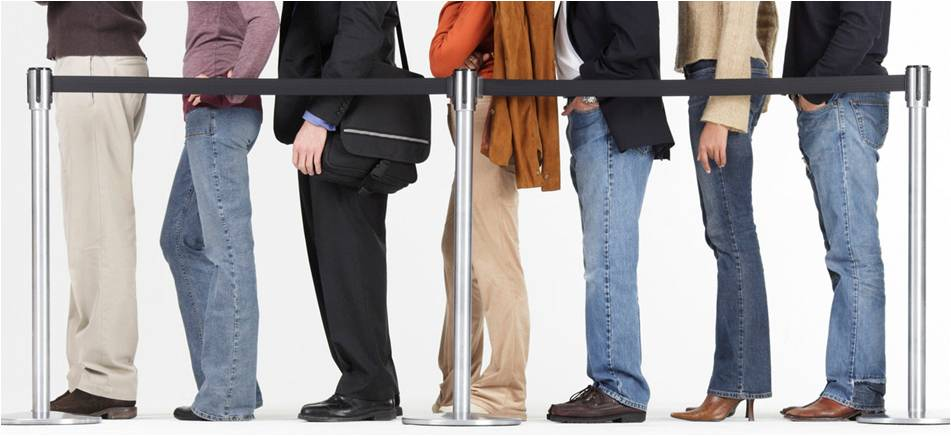
\includegraphics[width=250pt]{imgs/introducao.jpg}
  \label{fig_introducao}
\end{figure}
\end{frame}

%------------------------------------------------

\begin{frame}
\frametitle{Roteiro} % Table of contents slide, comment this block out to remove it
\tableofcontents % Throughout your presentation, if you choose to use \section{} and \subsection{} commands, these will automatically be printed on this slide as an overview of your presentation
\end{frame}

%----------------------------------------------------------------------------------------
%	PRESENTATION SLIDES
%----------------------------------------------------------------------------------------

%------------------------------------------------
\section{Objetivos}

\begin{frame}
\frametitle{Objetivos}

Esta aula tem como objetivos:

\begin{enumerate}
\item Apresentar os conceitos básicos sobre filas, pilhas e listas;
\item Explicitar as diferenças, vantagens e desvantagens de cada um;
\item Exemplificar os algoritmos por meio de pseudo-códigos.
\end{enumerate}

\end{frame}

%------------------------------------------------

\section{Referências bibliográficas}
  \frame{\frametitle{Referências bibliográficas}
    \bibliographystyle{abntex2-alf}
    \bibliography{referencias}
  }
  
%------------------------------------------------
\section{Introdução} % Sections can be created in order to organize your presentation into discrete blocks, all sections and subsections are automatically printed in the table of contents as an overview of the talk
%------------------------------------------------

\begin{frame}
\frametitle{Introdução}
\begin{itemize}
 \item As estruturas de dados são formas de distribuir e relacionar os dados disponíveis, de modo a tornar mais eficientes os algoritmos que manipulam esses dados;
 \item Quando o programador cria um algoritmo para solucionar um problema, ele também cria uma estrutura de dados que é manipulada pelo algoritmo.
\end{itemize}
\end{frame}

%------------------------------------------------

\begin{frame}
\frametitle{Introdução}

\begin{itemize}
 \item A escolha de uma determinada estrutura pode afetar substancialmente a quantidade de área de armazenamento requerida para o processamento bem como o tempo deste processamento;
 \item É, portanto, de grande importância o estudo de diferentes estruturas que possam ser utilizadas eventualmente na resolução de um problema, de forma a simplificar a sua implementação prática.
\end{itemize}
\end{frame}

%-----------------------------------------------
\section{Implementação Estática}
%------------------------------------------------

\subsection{Pilhas}

\begin{frame}
\frametitle{Implementação Estática}
\framesubtitle{Pilhas}
\centering
\huge{Implementação Estática\\
Pilhas
}
\end{frame}


\begin{frame}
\frametitle{Pilhas}
\begin{block} {Pilha}
 Segundo \citeonline{Ziviani2011}, uma pilha é uma lista linear em que todas as inserções, retiradas e todos os acessos são feitos em apenas um extremo da lista.
\end{block}

\begin{itemize}
 \item Adotam a política {\bf LIFO} (Last In, First Out) para manipulação de elementos; 
 \item Inserções e retiradas são realizadas no topo.
 \end{itemize}
\begin{figure}[!h]
  \centering
  
\includegraphics[width=100pt]{imgs/pilha.jpg}
  \label{fig_pilha}
\end{figure}
\end{frame}

%------------------------------------------------

\begin{frame}
\frametitle{Pilhas - Aplicações}
\begin{itemize}
 \item Ideal para estruturas aninhadas (verificação de parênteses, controle de sequências de subprogramas e etc.);
 \item Armazenar histórico de ações realizadas (páginas visitadas em um navegador, controle de destazer/refazer em um editor de testos);
 \item Utilizadas para implementar a recursividade (pilha de recursão).
\end{itemize}
\end{frame}

%------------------------------------------------

\begin{frame}
\frametitle{Pilhas - Operações básicas}
\begin{figure}[!h]
  \centering
  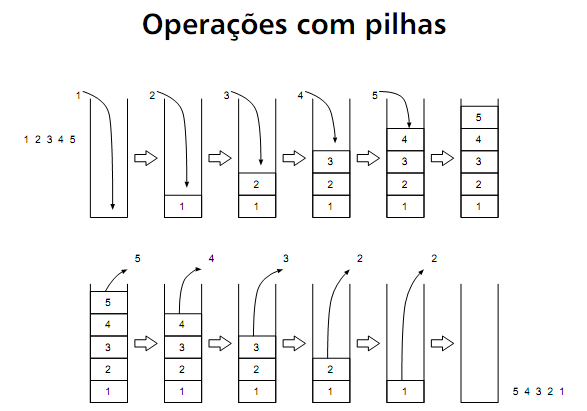
\includegraphics[width=250pt]{imgs/operacoes_pilhas.png}
  \label{fig_operacoes_pilhas}
\end{figure}
\end{frame}

%------------------------------------------------

\begin{frame}
\frametitle{Pilhas - Operações básicas}
\begin{enumerate}
 \item CriaPilhaVazia($S$) 
 \item PilhaVazia($S$)
 \item Empilha($S$,$x$)
 \item Desempilha($S$) 
\end{enumerate}
\end{frame}

%------------------------------------------------

\begin{frame}
\frametitle{Pilhas - Implementação com arranjo}
\begin{figure}[!h]
  \centering
  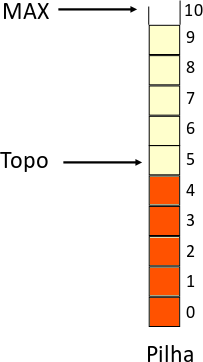
\includegraphics[width=100pt]{imgs/pilha_implementacao.png}
  \label{fig_pilha_implementacao}
\end{figure}
\end{frame}


%------------------------------------------------


\begin{frame}
\frametitle{Pilhas - Implementação com arranjo}

\begin{algorithm}[H]
\caption{CriaPilhaVazia} 
\label{CriaPilhaVazia}
\Entrada{Pilha $S$}
\Inicio{
  $S$.topo $\leftarrow$ 0 \\
}
\end{algorithm}

% \scalebox{0.5}{
\begin{algorithm}[H]
\caption{PilhaVazia} 
\label{PilhaVazia}
\Entrada{Pilha $S$}
\Saida{Booleano informando se $S$ está vazia}
\Inicio{
  \Se { ($S$.topo = 0) } {
    \Retorna Verdadeiro \\
    }
  \Senao {
    \Retorna Falso
  } 
}
\end{algorithm}
% }  
\tiny{ Adaptado de \citeonline{Cormen2012} e \citeonline{Ziviani2011}.}
\end{frame}

%------------------------------------------------

\begin{frame}
\frametitle{Pilhas - Implementação com arranjo}
% \scalebox{0.5}{
\begin{algorithm}[H]
\caption{Empilhar} 
\label{Empilhar}
\Entrada{Pilha $S$, item $x$ a ser empilhado}
\Inicio{
  \Se {($S$.topo = $S$.tamanhoMáximo)} {
      {\bf Erro } {\it overflow:} pilha cheia.
  }
  \Senao {
      $S$.itens[$S$.topo] $\leftarrow$ x \\
      $S$.topo $\leftarrow$ $S$.topo + 1 \\      
  }
}
\end{algorithm}
% }  
\tiny{ Adaptado de \citeonline{Cormen2012} e \citeonline{Ziviani2011}.}
\end{frame}

%------------------------------------------------

\begin{frame}
\frametitle{Pilhas - Implementação com arranjo}
% \scalebox{0.5}{
\begin{algorithm}[H]
\caption{Desempilhar} 
\label{Desempilhar}
\Entrada{Pilha $S$}
\Saida{Elemento desempilhado}
\Inicio{
  \Se { (PilhaVazia($S$)) } {
      \Retorna {\it underflow: } pilha vazia.
  } 
  \Senao {
      $x \leftarrow S$.itens[ $S$.topo - 1]\\
      $S$.topo $\leftarrow S$.topo - 1\\
      \Retorna $x$      
  }
}
\end{algorithm}
% }  
\tiny{ Adaptado de \citeonline{Cormen2012} e \citeonline{Ziviani2011}.}
\end{frame}

%------------------------------------------------
\subsection{Filas}
%------------------------------------------------

\begin{frame}
\frametitle{Implementação Estática}
\framesubtitle{Filas}
\centering
\huge{Implementação Estática\\
Filas
}
\end{frame}


\begin{frame}
\frametitle{Filas}
\begin{block}{Fila}
 De acordo com \citeonline{Ziviani2011}, uma fila é uma lista linear em que todas as inserções são realizadas em um extremo da lista, e todas as retiradas e acessos são realizados no outro extremo da lista.
\end{block}

\begin{itemize}
 \item Adotam a política {\bf FIFO} (First In, First Out) para manipulação de elementos;
 \item Inserções são realizadas no final da fila;
 \item Remoções são realizadas no início da fila.
\end{itemize}

\begin{figure}[!h]
%   \flushright
  \centering
  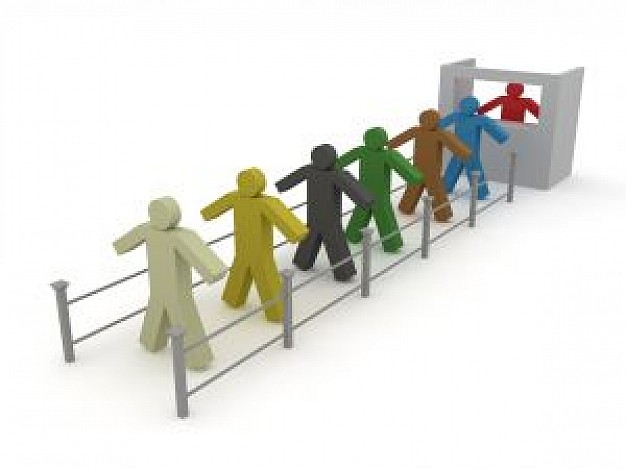
\includegraphics[width=100pt]{imgs/fila.jpg}
  \label{fig_fila}
\end{figure}

\end{frame}

%------------------------------------------------

\begin{frame}
\frametitle{Filas - Aplicações}
\begin{itemize}
 \item Alocação de recursos para impressão de documentos em uma impressora;
 \item Atendimento de processos requisitados ao sistema operacional;
 \item Ordenação do encaminhamento de pacotes em um roteador;
 \item Buffer para gravação de dados em mídia.
\end{itemize}
\end{frame}

%------------------------------------------------

\begin{frame}
\frametitle{Filas - Operações básicas}
\begin{enumerate}
 \item CriaFilaVazia($Q$) 
 \item FilaVazia($Q$)
 \item Enfileira($Q$,$x$)
 \item Desenfileira($Q$) 
\end{enumerate}
\end{frame}

%------------------------------------------------

\begin{frame}
\frametitle{Filas - Operações básicas}
\begin{figure}[!h]
  \centering
  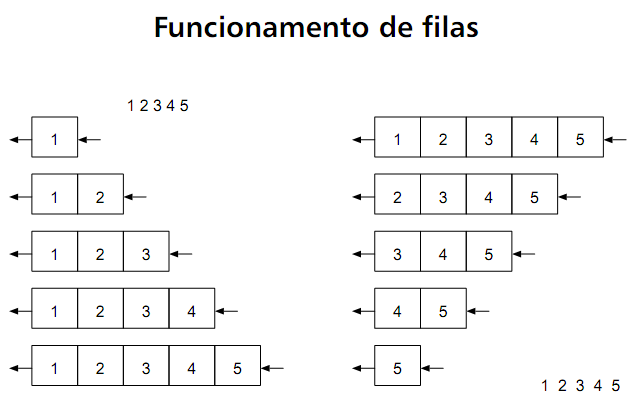
\includegraphics[width=250pt]{imgs/operacoes_filas.png}
  \label{fig_operacoes_filas}
\end{figure}
\end{frame}

%------------------------------------------------

\begin{frame}
\frametitle{Filas - Implementação com arranjo}
\begin{figure}[!h]
  \centering
  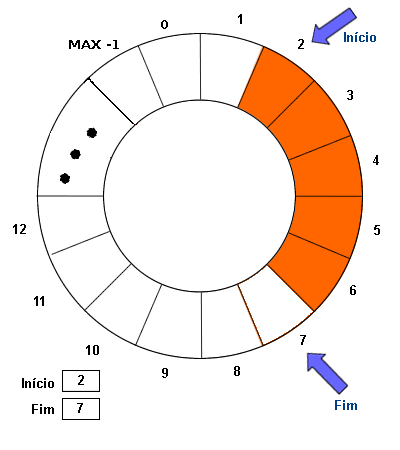
\includegraphics[width=150pt]{imgs/fila_implementacao.png}
  \label{fig_fila_implementacao}
\end{figure}
\end{frame}

\begin{frame}
\frametitle{Filas - Implementação com arranjo}
\begin{figure}[!h]
  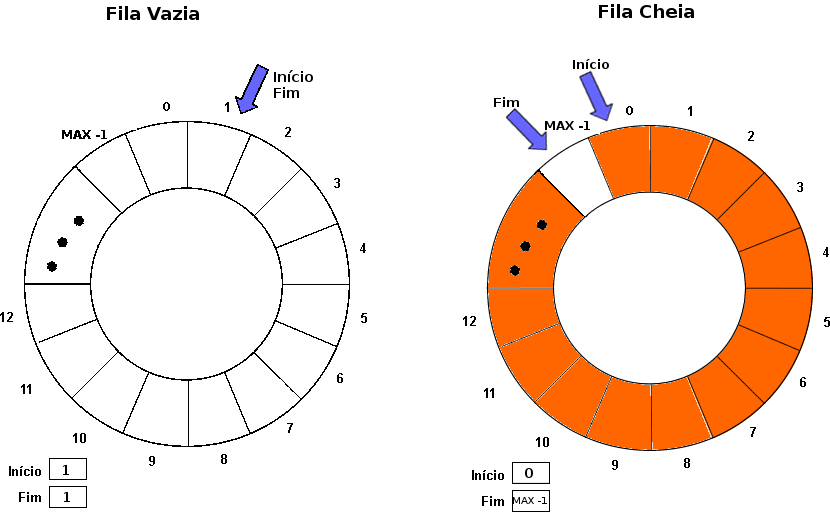
\includegraphics[width=300pt]{imgs/fila_estados.png}
\end{figure}
\end{frame}

%------------------------------------------------

\begin{frame}
\frametitle{Fila - Implementação com arranjo}
% \scalebox{0.5}{
\begin{algorithm}[H]
\caption{CriaFilaVazia} 
\label{CriaFilaVazia}
\Entrada{Fila $Q$}
\Inicio{
  $Q$.início $\leftarrow$ 0 \\
  $Q$.fim $\leftarrow$ $Q$.início \\
}
\end{algorithm}
% }  
\begin{algorithm}[H]
\caption{FilaVazia} 
\label{FilaVazia}
\Entrada{Fila $Q$.}
\Inicio{
  \Se {($Q$.início = $Q$.fim)} {
      \Retorna Verdadeiro 
  }
  \Senao {
      \Retorna Falso
  }
}
\end{algorithm}
\tiny{ Adaptado de \citeonline{Cormen2012} e \citeonline{Ziviani2011}.}
\end{frame}

%------------------------------------------------

\begin{frame}
\frametitle{Fila - Implementação com arranjo}
% \scalebox{0.5}{
\begin{algorithm}[H]
\caption{Enfileira} 
\label{Enfileira}
\Entrada{Fila $Q$, item $x$}
\Inicio{
  \Se { ( ($Q$.fim) MOD ($Q$.tamanhoMáximo) + 1 = $Q$.início)} {
      {\bf Erro }{\it overflow}: fila cheia.
  }
  \Senao {
      $Q$.itens[$Q$.fim] $\leftarrow$ x \\
      $Q$.fim $\leftarrow$ ($Q$.fim) MOD ($Q$.tamanhoMáximo) + 1 \\
  }
}
\end{algorithm}

\tiny{ Adaptado de \citeonline{Cormen2012} e \citeonline{Ziviani2011}.}
\end{frame}


%------------------------------------------------

\begin{frame}
\frametitle{Fila - Implementação com arranjo}
% \scalebox{0.5}{
\begin{algorithm}[H]
\caption{Desenfileira} 
\label{Desenfileira}
\Entrada{Fila $Q$}
\Saida{Elemento desenfileirado}
\Inicio{
  \Se {FilaVazia($Q$)} {
      \Retorna Erro {\it underflow}: fila vazia. 
  }
  \Senao {
      $x$ $\leftarrow$ $Q$.itens[$Q$.início] \\
      $Q$.início $\leftarrow$ ($Q$.início) MOD ($Q$.tamanhoMáximo) + 1 \\
      \Retorna $x$
      
  }
}
\end{algorithm}
% }  
\tiny{ Adaptado de \citeonline{Cormen2012} e \citeonline{Ziviani2011}.}
\end{frame}

%------------------------------------------------
\subsection{Listas}
%------------------------------------------------


\begin{frame}{Implementação Estática}{Listas}
\centering
\huge{Implementação Estática\\
Listas
}
\end{frame}


\begin{frame}
\frametitle{Listas}
\begin{block}{Lista}
Na lista, ao inserir ou remover elementos não existe nenhuma restrição, podendo realizar uma determinada operação em qualquer posição.
\end{block}
\begin{itemize}
 \item Ao inserir um elemento em uma posição, é necessário deslocar os elementos para que nenhum elemento seja sobreposto.
 \item Ao remover um elemento é necessário deslocar os elementos de modo a ocupar a posição vazia.
\end{itemize}
\begin{figure}[!h]
  \centering
  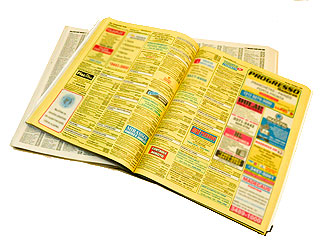
\includegraphics[width=100pt]{imgs/lista.jpg}
  \label{fig_lista}
\end{figure}
\end{frame}


%------------------------------------------------

\begin{frame}
\frametitle{Listas - Operações básicas}
\begin{enumerate}
 \item CriaListaVazia($L$) 
 \item ListaVazia($L$)
 \item Inserir($L$, $x$, $p$)
 \item Remover($L$, $p$) 
\end{enumerate}
\end{frame}

%------------------------------------------------

\begin{frame}
\frametitle{Lista - Implementação com arranjo}
% \scalebox{0.5}{
\begin{algorithm}[H]
\caption{CriaListaVazia} 
\label{CriaListaVazia}
\Entrada{Lista $L$}
\Inicio{
  $L$.primeiro $\leftarrow$ 0 \\
  $L$.ultimo $\leftarrow$ $L$.primeiro \\
}
\end{algorithm}
% }  
\begin{algorithm}[H]
\caption{ListaVazia} 
\label{ListaVazia}
\Entrada{Lista $L$.}
\Inicio{
  \Se {($L$.primeiro = $L$.ultimo)} {
      \Retorna Verdadeiro 
  }
  \Senao {
      \Retorna Falso
  }
}
\end{algorithm}
\tiny{ Adaptado de \citeonline{Cormen2012} e \citeonline{Ziviani2011}.}
\end{frame}

%------------------------------------------------

\begin{frame}
\frametitle{Lista - Implementação com arranjo}
% \scalebox{0.5}{
\begin{algorithm}[H]
\caption{Inserir} 
\label{Inserir}
\Entrada{Lista $L$, elemento $x$, posição $p$}
\Inicio{
  \Se { ( ($L$.ultimo + 1) MOD $L$.tamanhoMáximo = $L$.primeiro )} {
      {\bf Erro }{\it overflow}: lista cheia.
  }
  \Senao {
      \Para {( $i \leftarrow L.ultimo $ até $p$) } { 
      	$L$.itens[ i+1 ] $\leftarrow$ $L$.itens[ i ] \\
      }
     	$L$.itens[ $p$ ] $\leftarrow$ x \\
     	$L$.ultimo = $L$.ultimo + 1 \\
  }
}
\end{algorithm}
\tiny{ Adaptado de \citeonline{Cormen2012} e \citeonline{Ziviani2011}.}
\end{frame}


%------------------------------------------------

\begin{frame}
\frametitle{Lista - Implementação com arranjo}
% \scalebox{0.5}{
\begin{algorithm}[H]
\caption{Remove} 
\label{Remove}
\Entrada{Lista $L$, posição $p$}
\Saida{Elemento removido}
\Inicio{
  \Se {ListaVazia($L$)} {
      \Retorna Erro {\it underflow}: lista vazia. 
  }
  \Senao {
    	$x$ $\leftarrow$ $L$.itens[ p ] \\
  	\Para {( $i \leftarrow p$ até $L.ultimo$ ) }  {
      	$L$.itens[ i ] $\leftarrow$ $L$.itens[ i+1 ] \\
     }
     $L$.ultimo = $L$.ultimo - 1 \\
     	\Retorna $x$
  }
}
\end{algorithm}
\end{frame}
%---------------------
%------------------------------------------------
\section{Conclusão}
%------------------------------------------------
\begin{frame}
\frametitle{Conclusão}
Conclusão
\begin{block} {Material de apoio}
 Animações das operações disponíveis em http://www.ime.usp.br/\~{ }nelio/ensino/2002-1/ed/
\end{block}
\begin{block} {Próxima aula}
 Pilha, Fila e Lista com alocação dinâmica.
\end{block}
\end{frame}


%------------------------------------------------

%\begin{frame}
%\Huge{\centerline{Dúvidas?}}
%
%\begin{figure}[!h]
%  \centering
%  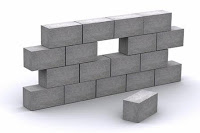
\includegraphics[width=100pt]{imgs/duvidas.jpg}
%  \label{fig_fim}
%\end{figure}
%
%\end{frame}

\begin{frame}
\titlepage % Print the title page as the first slide

\begin{figure}[!h]
  \centering
  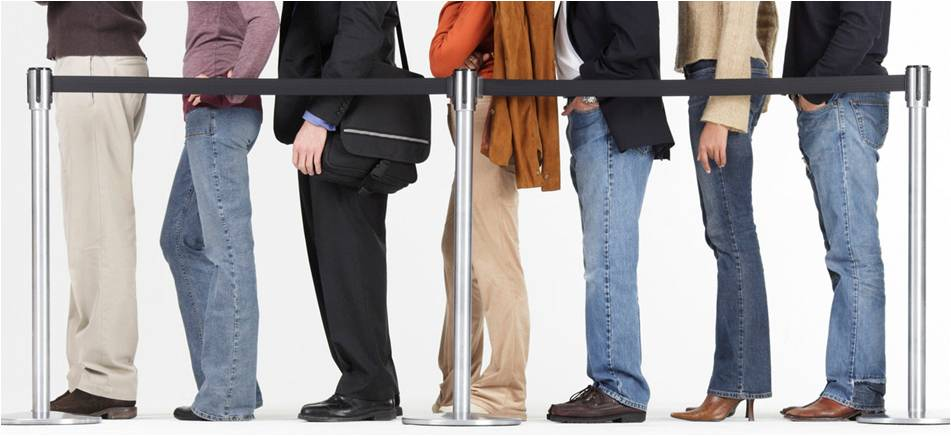
\includegraphics[width=250pt]{imgs/introducao.jpg}
  \label{fig_introducao}
\end{figure}
\end{frame}


%----------------------------------------------------------------------------------------


\end{document} 